\documentclass[main.tex]{subfiles}

\begin{document}

% \textcolor{red}{Вводная лекция}

\section{Лекция 16.02.2021 (Донцов Е.В.)}

План на сегодня: рассказать про основные компоненты моделирования ГРП (HF = hydraulic fracturing), про основные используемые уравнения и основные геометрии.

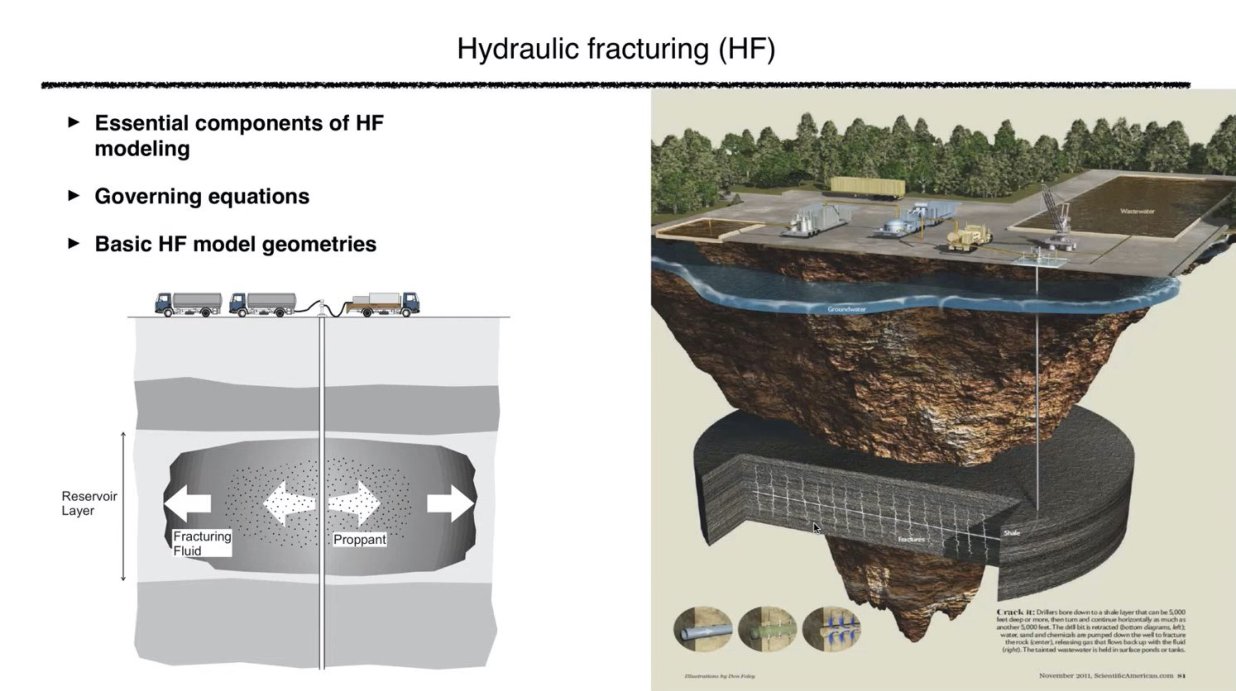
\includegraphics[width=\textwidth, page=1]{HF_slides.pdf}

В двух словах разница между conventional и unconventional:

1) conventional -- то, что было, грубо говоря, до 2000-х годов -- вертикальная скважина, пласт, рвём гидроразрывом пласта, обычно одна трещина;

2) unconventional -- когда сланцы, например, то бурится горизонтальная скважина, проводится многостадийный ГРП (за одну стадию можем сделать несколько трещин (несколько портов), затем поставить перегородку, сделать ещё несколько трещин (портов) и так далее); можем также сделать несколько скважин.

Концептуально с точки зрения математики разницы между conventional и unconventional практически нет.
У нас либо одна трещина (conventional) или множество трещин (unconventional), т.е. с точки зрения моделирования unconventional моделировать дольше, сложнее.
Но повторюсь, что концептуально основная физика везде одинакова.

\subsection{Из чего состоит любая модель ГРП? Основные компоненты}

\includegraphics[width=\textwidth, page=2]{HF_slides.pdf}

Основные компоненты любой модели гидроразрыва пласта:

1) закон сохранения жидкости; в 99\% случаев предполагается, что жидкость несжимаема, тогда выполняется закон сохранения объёма; но бывают случаи сжимаемых жидкостей (например, когда ГРП делают газом или делают пенный ГРП), тогда выполняется закон сохранения массы, т.е. закачиваемый объём жидкости равен объёму жидкости в трещине плюс утечки (трещину ГРП делаем в пористом резервуаре, поэтому есть утечки из трещины в резервуар -- в зависимости от пористости и других параметров утечки могут либо доминировать, либо нет: например, 90\% закачиваемой жидкости может утекать в пласт или наоборот оставаться в трещине);

2) уравнение течения жидкости в трещине;
допустим мы уже создали трещину в резервуаре (обычно она очень узкая и длинная: например, 1 сантиметр в ширину и порядка сотни метров в длину) и закачиваем в неё жидкость (которая часто бывает довольно вязкой), тогда у нас может быть существенное падение давления от скважины до кончика трещины (так как грубо говоря, всю эту жидкость нужно пропихнуть по всей трещине);
необходимы уравнения течения жидкости в зависимости от реологии жидкости;

3) равновесие (упругость) горной породы;
когда мы открываем трещину в упругом материале, то мы предполагаем, что порода линейно упругая (по крайней мере в первом приближении);
чтобы открыть трещину (т.е. просто открыть (как надуть шарик), а не распространить), нам необходимо приложить какое-то давление на стенки трещины (это давление и есть давление жидкости внутри трещины);
у нас получается некое распределение давления внутри трещины, и оно как-то неравномерно открывает эту трещину; чем сильнее мы хотим открыть трещину, тем больше должно быть давление жидкости внутри;

концептуальное уравнение: Fluid Pressure = Stress + Stiffness * FracWidth -- давление жидкости должно превысить напряжение в породе + жёсткость трещины (которая напрямую зависит от модуля Юнга породы), умноженную на среднее открытие трещины;
но большую часть составляет именно напряжение в породе, а дополнительное слагаемое с жёсткостью обычно много меньше (но тем не менее очень важно для моделирования); 

4) условие распространения трещины; грубо говоря, продолжая аналогию с шариком -- это критерий, при котором шарик лопнет; при достижении критического значения некого параметра около кончика трещины начнётся распространение трещины;

5) транспорт проппанта; это тоже очень важный компонент физики модели ГРП; высокопроводимый проппант нужен для того, чтобы при смыкании трещины ГРП остались проводимые каналы;
с точки зрения моделирования внутри жидкости течёт суспензия; обычно частицы проппанта (часто используется песок или керамический проппант с примерной плотностью 2.65 г/см$^3$) тяжелее жидкости (у воды плотность приблизительно 1 г/см$^3$), поэтому интересно моделировать процесс оседания проппанта.

\subsection{Модель утечки по Картеру}

\includegraphics[width=\textwidth, page=3]{HF_slides.pdf}

Давайте рассмотрим модель утечки по Картеру.
Эта модель является доисторической для рассматриваемой области (для моделирования ГРП), её развил Картер ещё в 1956-1957 годах (тогда ещё только зарождался ГРП).
Первый коммерческий ГРП был сделан примерно в 1950-х годах.
Но тем не менее модель Картера и сейчас очень часто (почти повсеместно) используется при моделировании ГРП, потому что она очень простая и очень много физики в себе несёт.

В левом верхнем углу на слайде изображен рисунок (из PhD диссертации J. Adachi), на котором изображена область вблизи трещины.
Обычно жидкость ГРП состоит из основной жидкости (base fluid) и полимеров (их добавляют, чтобы химия или реология совпадала с той, которая нужна для дизайна ГРП, например, для нужной длины трещины или нужного транспорта проппанта и так далее).
Идея в том, что есть жидкость с полимерами.
Когда эта жидкость начинает фильтроваться в породу, то происходит следующее: в классической модели считаем, что полимеры большие, длинные и с трудом залезают в поровое пространство, т.е. полимеры в основном осаждаются на стенке трещины.
В итоге, образуется Filter Cake, который состоит из полимеров, добавляемых в жидкость ГРП.

Далее идёт Invaded Zone, в которой жидкость ГРП без полимеров затекает в породу и вымещает жидкость резервуара.

Далее идёт сам резервуар, в котором давление поднялось (так как мы вытеснили часть жидкости из Invaded Zone в резервуар).

Таким образом, концептуально график зависимости давления от вертикальной координаты $y$ выглядит следующим образом: на стенке трещины давление равно давлению жидкости, на бесконечности -- давление резервуара; 
давление жидкости больше, чем давление резервуара (иначе не смогли бы сгенерировать трещину ГРП);
есть падение давления на корке Filter Cake (предполагается, что оно линейное);
есть падение давления в Invaded Zone (тоже предполагается, что оно линейное);
и дальше есть падение давления в резервуаре.

Итак, есть три характерных падения давления.
Может быть так, что какое-то из них много меньше, чем другое; какое-то давление доминирует; может быть отсутствие Filter Cake (если в жидкости ГРП нет полимеров).
Но мы рассмотрим более общий случай и пройдёмся по уравнениям.

На слайде в левом нижнем углу представлена картина пористости сланца, полученная с помощью электронного микроскопа (маленькие поры, различные минералы и видно, что через эти поры жидкость утекает).
\\

Первым делом рассмотрим течение через корку Filter Cake.


\includegraphics[width=\textwidth, page=4]{HF_slides.pdf}

\includegraphics[width=\textwidth, page=5]{HF_slides.pdf}

\subsection{Течение жидкости}

\includegraphics[width=\textwidth, page=6]{HF_slides.pdf}

\subsection{Равновесие (упругость) горной породы}

\includegraphics[width=\textwidth, page=7]{HF_slides.pdf}



\end{document}